\usepackage[latin1]{inputenc}
\usepackage{array}
\usepackage{amsmath}
\usepackage{upgreek}
\usepackage{hyperref}

\usepackage{minted}
\usemintedstyle{perldoc}
\newmintedfile{c}{fontsize=\tiny, frame=lines, framesep=1mm}

\usepackage[absolute,overlay]{textpos}

\usepackage{media9}

\setbeamercolor{framesource}{fg=gray}
\setbeamerfont{framesource}{size=\tiny}

\newcommand{\source}[1]{\begin{textblock*}{4cm}(8.7cm,8.6cm)
    \begin{beamercolorbox}[ht=0.5cm,right]{framesource}
        \usebeamerfont{framesource}\usebeamercolor[fg]{framesource} Image Source: {#1}
    \end{beamercolorbox}
\end{textblock*}}

% \usepackage{minted}
% \usemintedstyle{perldoc}
% tiny, scriptsize, footnotesize, small, normalsize, large, Large, LARGE,
% huge Huge
% \newminted{d}    {fontsize=\tiny, frame=lines, framesep=1mm}
% \newminted{bash} {fontsize=\tiny, frame=lines, framesep=1mm}
% \newmintedfile{d}{fontsize=\tiny, frame=lines, framesep=1mm}

\usetheme[numbers, minimal]{NYU}
% Get rid of the navigation icons
\setbeamertemplate{navigation symbols}{}

\title{Mesh-Free FEM \\ for Structural Analysis and Optimization}
\author{Julian Panetta}
\date{8 October 2013}
\begin{document}

\begin{frame}
\titlepage
\end{frame}

\section{Worst-Case Structural Analysis}
\begin{frame}{Worst-Case Structural Analysis}
    \begin{itemize}
        \item Siggraph '13 Pipeline:
            \begin{figure}
                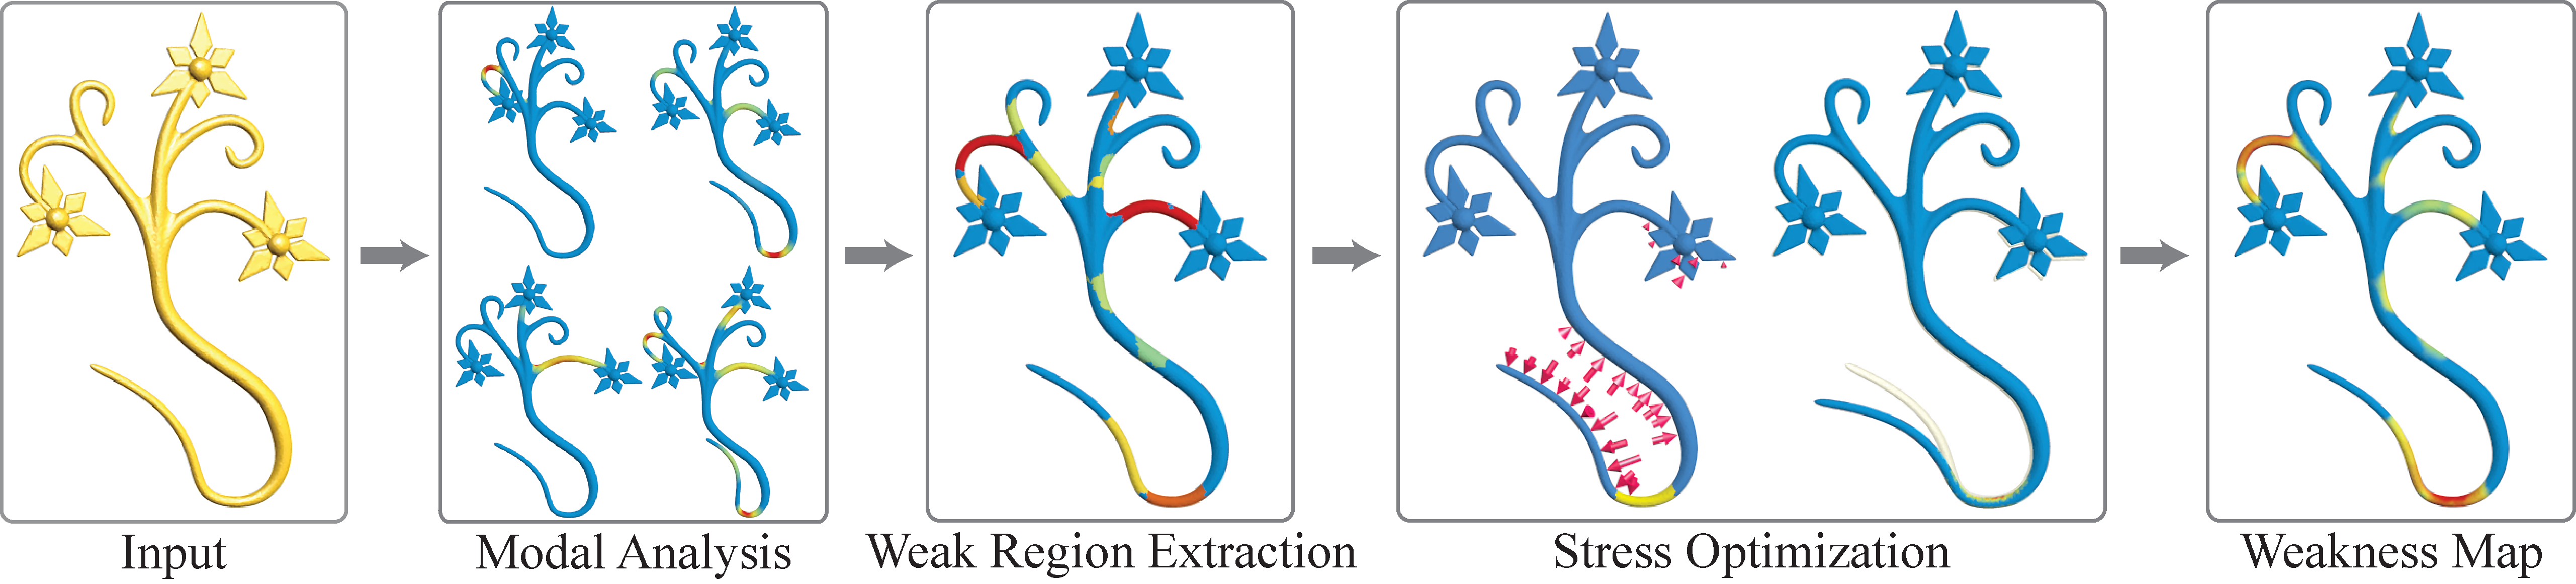
\includegraphics[width=.9\textwidth]{images/algorithm_overview.pdf}
            \end{figure}
        \pause \item Hidden initial stage: volume meshing!
        \pause \item Volume meshing is undesirable in many ways.
    \end{itemize}
\end{frame}

\begin{frame}{Mesh-free: Why?}
    \begin{itemize}
        \item Complicated geometry can be hard to mesh robustly.
            \begin{figure}
                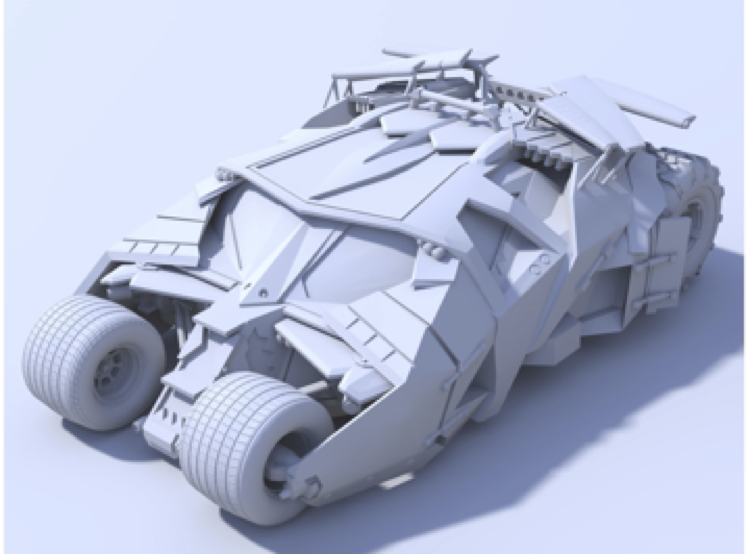
\includegraphics[width=.3\textwidth]{images/batmobile.png}
            \end{figure}
        \pause \item Free ourselves from the surface resolution \\(e.g., we might want
                     to coarsen some regions).
        \pause \item Sometimes you don't even have a boundary mesh (CSG)
            \begin{figure}
                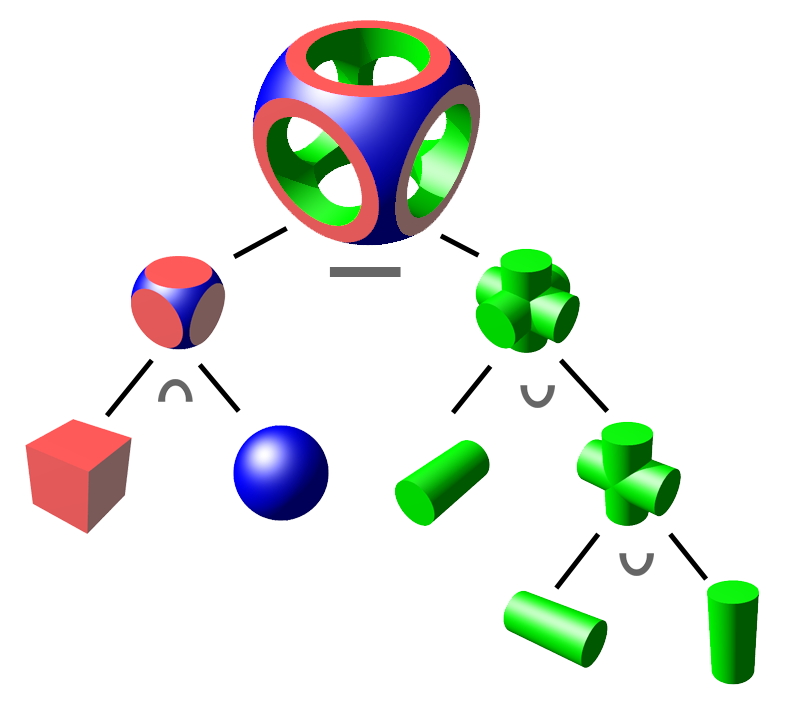
\includegraphics[width=.3\textwidth]{images/csg_tree.png}
                \source{Wikipedia}
            \end{figure}
    \end{itemize}
\end{frame}

\begin{frame}{Mesh-free: Why?}
    \begin{itemize}
        \item Results are often mesh-dependent:
            \begin{figure}
                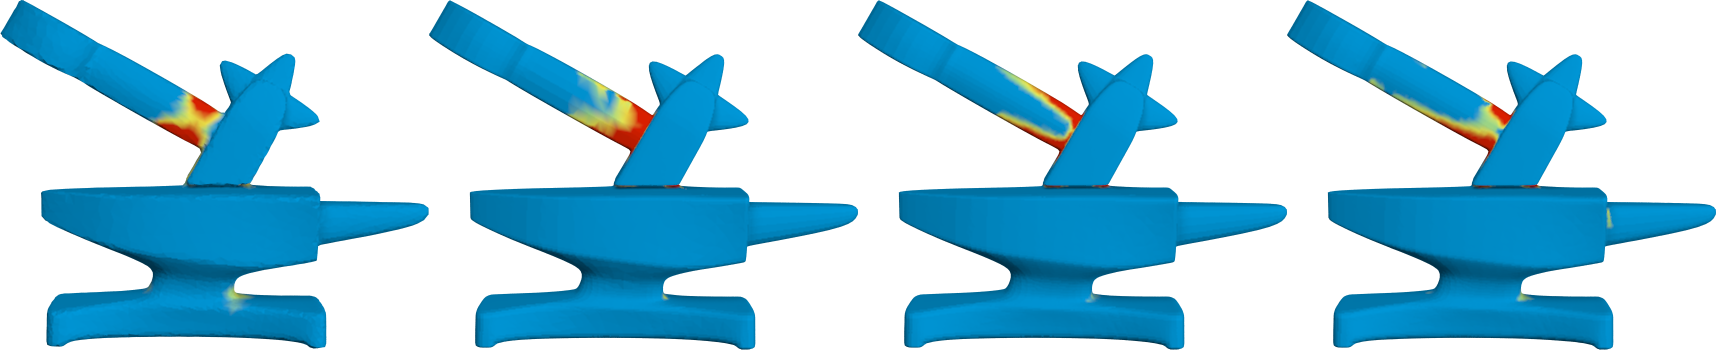
\includegraphics[width=.8\textwidth]{images/mesh_dep.png}
            \end{figure}
            We want a methodical way to study/correct for this.
        \pause \item Everything is much worse when iteratively
            tweaking shapes:
            \begin{itemize}
        \pause  \item Remeshing after each tweak is expensive and could fail.
        \pause  \item A small tweak could trigger a different meshing with
                      qualitatively different results.
            \end{itemize}
    \end{itemize}
\end{frame}

\begin{frame}{Mesh-free: What?}
    \begin{itemize}
        \item Use FEM discretization, but only query geometry through
              inside/outside tests and boundary point lists.
              
        \pause \item There *is* still a mesh: a regular grid.
            \begin{figure}
                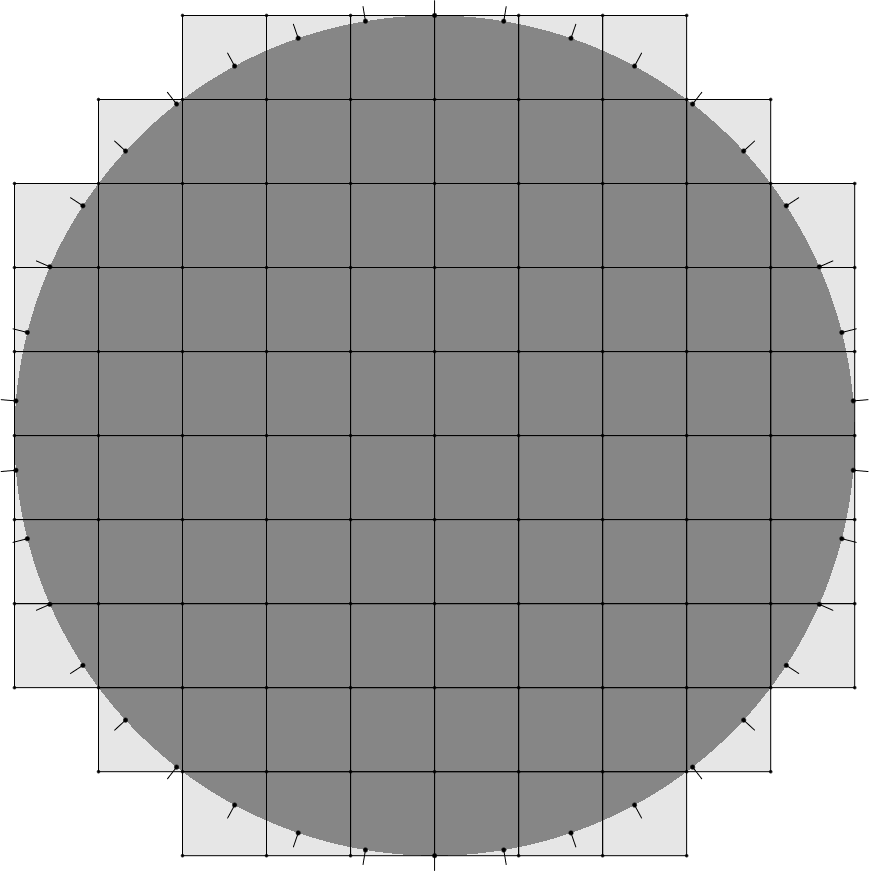
\includegraphics[width=.4\textwidth]{images/meshfree.png}
            \end{figure}
        \pause \item Note: doesn't conform to the object's boundary.
    \end{itemize}
\end{frame}

\begin{frame}{Linear Elasticity}
    \begin{itemize}
        \item This talk will focus on the discretization of the (2D) linear
              elasticity equations; the rest of the pipeline is straightforward.
 \pause \item Elastostatic equation (force balance):
     \begin{align*}
         \nabla \cdot \sigma + {\bf F}_v &= 0 &\text{in }\Omega \\
         \sigma {\bf \hat{n}} &= {\bf F}_b &\text{on }\partial \Omega
    \end{align*}
    $\sigma$ stress tensor (matrix), ${\bf F}_v$ and ${\bf F}_b$ volume
    and boundary forces (vector fields), ${\bf \hat{n}}$ surface normal
        \pause \item Solve for displacement field, ${\bf u},$ where:
        \begin{align*}
            \sigma_{ij} = C_{ijkl} \epsilon_{ij} = \frac{1}{2} C_{ijkl}
            \left(\left[\nabla {\bf u}\right]_{ij} + \left[\nabla {\bf u}\right]_{ji}\right)
        \end{align*}
    \pause \item (whiteboard picture)
    \end{itemize}
\end{frame}

\begin{frame}{FEM Discretization}
        Following the standard FEM procedure, we use the weak form:
            \begin{align*}
                \int_\Omega \! (\nabla \cdot \sigma) \cdot {\bf v}\, \mathrm{d}x
                = -\int_{\Omega} \! {\bf F}_v \cdot {\bf v}\, \mathrm{d}x \quad
                \forall {\bf v}: \mathbb{R}^2 \to \mathbb{R}^2,
            \end{align*}
            Integrating by parts, applying boundary conditions, using basis
            functions ${\bf \phi}_i$ for both test and trial functions, and
            ``flattening'' tensors, we get a linear system:
     \pause \begin{align*}
                \underbrace{\left( \int_{\Omega} \! B^T D B \, \mathrm{d}x \right)}_{K} {\bf u}_h = 
                \int_{\partial \Omega} \! {\bf \phi}_i \cdot {\bf F}_b\, \mathrm{d}S + 
                \int_{\Omega} \! {\bf \phi}_i \cdot {\bf F}_v\, \mathrm{d}x,
            \end{align*}
            $K$ ``stiffness matrix'' maps nodal displacements to nodal forces \\
            $B$, a matrix of $\phi_i$ gradients, maps displacement to strain \\
            $D$ maps strain to stress (depends only on material properties)
            ${\bf u}_h = (u_{1x}, u_{1y}, ..., u_{nx}, u_{ny})^T$ flattened per-node displacement
\end{frame}

\begin{frame}{Bilinear Quad Discretization}
    \begin{itemize}
        \item That derivation was for general basis functions.
 \pause \item My 2D implementation uses bilinear quad elements. \\
              These have a quadratic basis function at each corner:
 \pause       $$
                  \phi_0 = (1 - x)(1 - y) \quad \phi_1 = x(1 - y) \quad \phi_2 = xy \quad \phi_3 = (1 - x)y
              $$

              \begin{figure}
                  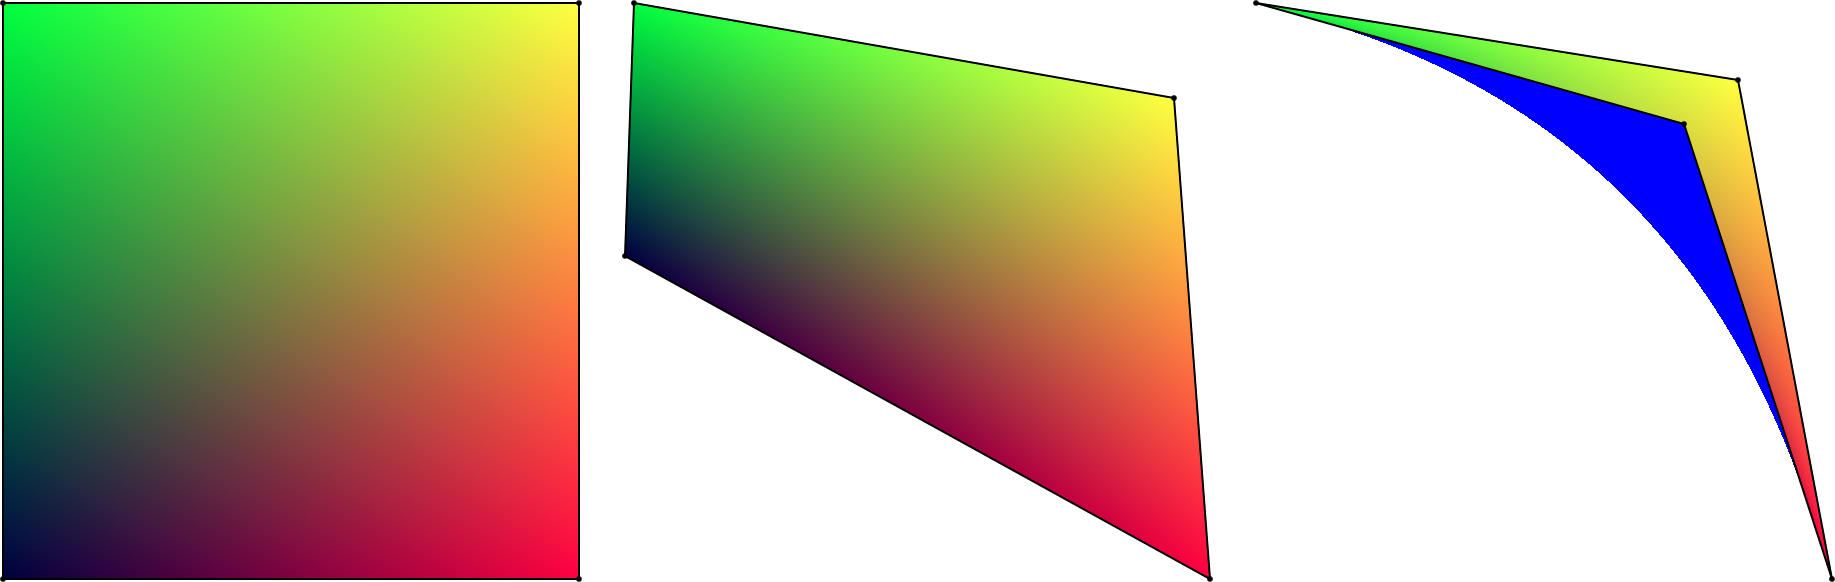
\includegraphics[width=.6\textwidth]{images/bilinear_quad.png}
                  \caption{Visualization of displacement interpolation. Non-bijective for concave quads.}
              \end{figure}
    \end{itemize}
\end{frame}

\begin{frame}{Building the System: The Stiffness Matrix}
            \begin{align*}
                \underbrace{\left( \int_{\Omega} \! B^T D B \, \mathrm{d}x \right)}_{K} {\bf u}_h = 
                \int_{\partial \Omega} \! {\bf \phi}_i \cdot {\bf F}_b\, \mathrm{d}S + 
                \int_{\Omega} \! {\bf \phi}_i \cdot {\bf F}_v\, \mathrm{d}x,
            \end{align*}

    \begin{itemize}
\pause  \item The stiffness matrix integral can be broken down into per-element integrals:
\pause      \begin{align*}
                K = \int_{\Omega} \! B^T D B \, \mathrm{d}x =
                \sum_e \int_{\Omega \cap e} \! B_e^T D B_e \, \mathrm{d}x := \sum_e K_e
            \end{align*}
            where $B_e$ only involves the gradients of the basis function sitting on cell $e$'s nodes.
        \pause \item $B_e$ is a linear function of ${\bf x}$, so the integrands are quadratic.
        \pause \item For cells completely overlapping the object, this integral has a closed form.
    \end{itemize}
\end{frame}

\begin{frame}{The Stiffness Matrix: Cut Cells}
    \begin{itemize}
        \item The difficulty comes in at the ``cut'' cells:
            \begin{figure}
                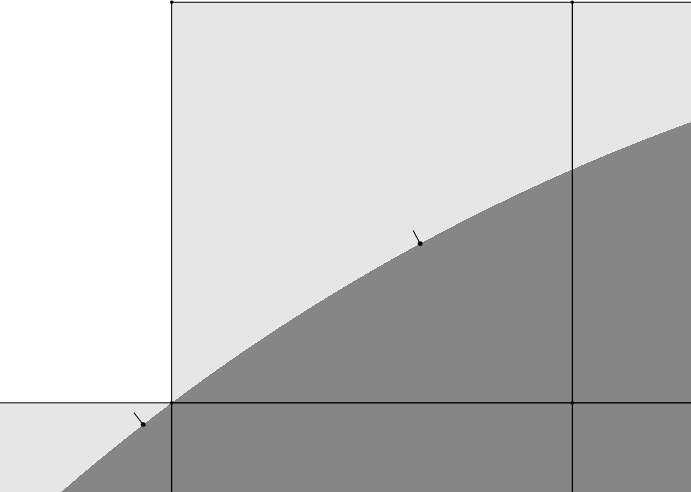
\includegraphics[width=.4\textwidth]{images/cut_cell.png}
            \end{figure}
 \pause \item Here we compute the integral
            $$
            \int_{\Omega \cap e} \! B_e^T D B_e \, \mathrm{d}x = 
            \int_{e} \! I_\Omega B_e^T D B_e \, \mathrm{d}x
            $$
            where $I_\Omega$ is the indicator function:
            \begin{align*}
            I_\Omega = \begin{cases} 1 & \mbox{if } x \in \Omega \\
                                     0 & \mbox{otherwise} \end{cases}
            \end{align*}
    \end{itemize}
\end{frame}

\begin{frame}{Integration}
    $$
    \int_{e} \! I_\Omega B_e^T D B_e \, \mathrm{d}x
    $$
    \begin{itemize}
        \item Integration for cut cells is done numerically. The integral
            converges reasonably with uniform quadrature even though the
            integrand is discontinuous.
            \begin{figure}
                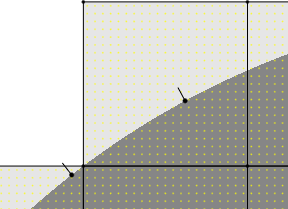
\includegraphics[width=.4\textwidth]{images/quadrature.png}
            \end{figure}
    \end{itemize}
\end{frame}

\begin{frame}{Boundary Integral}
    \begin{itemize}
        \item We also need the boundary integral (to apply forces):
            $$
            \int_{\partial \Omega} \! {\bf \phi}_i \cdot {\bf F}_b\, \mathrm{d}S
            $$
 \pause \item We only know the forces at boundary points.
 \pause \item Could treat ${\bf F}_b$ as a sum of delta functions at these
              points, but this is unrealistic (pin pricks).
 \pause \item Ideally we'd smoothly interpolate between boundary
              points.
 \pause \item We do this volumetrically, blurring the boundary force
     into a volume force, ${\bf F}_v = \sum_p \psi_p({\bf x}) {\bf F}_b(p)$
            \begin{figure}
                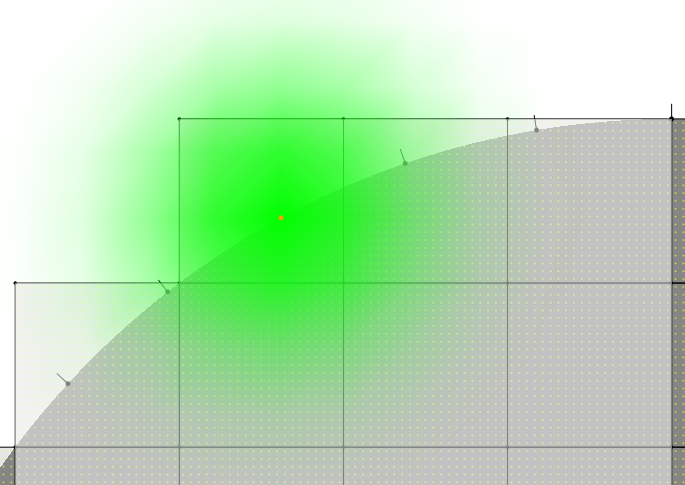
\includegraphics[width=.4\textwidth]{images/force_blur.png}
            \end{figure}

    \end{itemize}
\end{frame}

\begin{frame}{Full System}
    \begin{itemize}
        \item Neglecting true volume forces (e.g. gravity), the discrete system becomes:
            $$
            K {\bf u}_h = {\bf f},
            $$
            where
            \begin{align*}
                K &= \sum_e \int_{e} \! I_\Omega B_e^T D B_e \, \mathrm{d}x \\
                {\bf f} &= \sum_e \int_{e} \left( \! I_\Omega \sum_p \psi_p {\bf F}_b(p) \right) \, \mathrm{d}x.
            \end{align*}
        \pause \item Given boundary forces, finding the deformation is now just a linear solve! (Though K has a nullspace of dimension 2...)
    \end{itemize}
\end{frame}

\begin{frame}{Mesh-free FEM: Miscellanea}
    \begin{itemize}
        \item This discretization also gives us per-element stress tensors,
            $$\sigma_e = \left(\frac{1}{|e|}\int_e \! D B_e \, \mathrm{d}x \right) {\bf u}_h$$
        \pause \item Visualization
            \begin{itemize}
                \pause \item Discretization gives displacements on the grid nodes
                \pause \item We must evaluate the interpolated displacement
                             field to deform the object itself
                \pause \item Solution: Fancy GLSL shader warping texture coordinates
            \end{itemize}
        \pause \item Demo
    \end{itemize}
\end{frame}

\begin{frame}{Structural Optimization}
    \begin{itemize}
        \item Traditionally divided into sizing/shape/topology optimization
 \pause \item For a given loading scenario,
              find a shape that, e.g.,
            \begin{itemize}
                \pause \item has minimal mass while not breaking
                \pause \item deforms minimally for a fixed total mass
                \pause \item etc.
            \end{itemize}
 \pause \item Representative approach for topology optimization:
            \begin{itemize}
                \pause \item Initialize with grid full of material
                \pause \item Simulate loading scenario
                \pause \item Remove material from lowest stress cell
                \pause \item Repeat until something breaks
            \end{itemize}
    \begin{figure}
        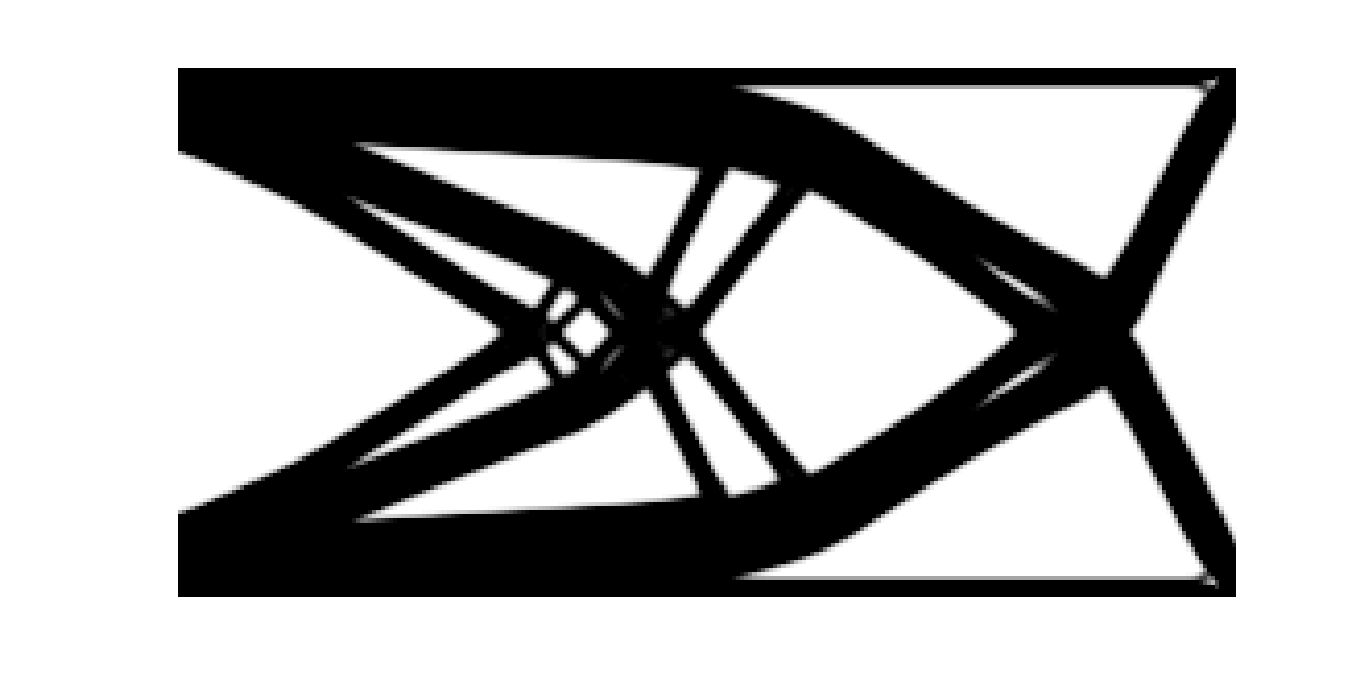
\includegraphics[width=.5\textwidth]{images/top_opt.png}
        \source{Wikipedia}
    \end{figure}
    \pause \item But, we can use our CSG representation to combine sizing/shape/topology optimization
    \end{itemize}
\end{frame}

\begin{frame}{CSG Structural Optimization}
        \begin{figure}
            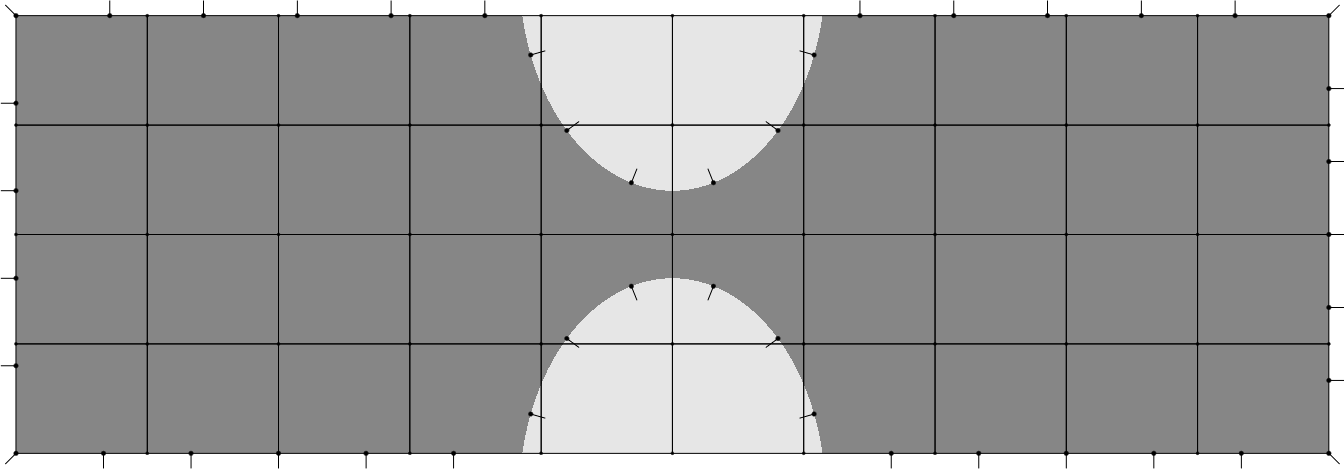
\includegraphics[width=.4\textwidth]{images/shape_opt1.png} \, \raisebox{.07\textheight}{$\Rightarrow$} \,
            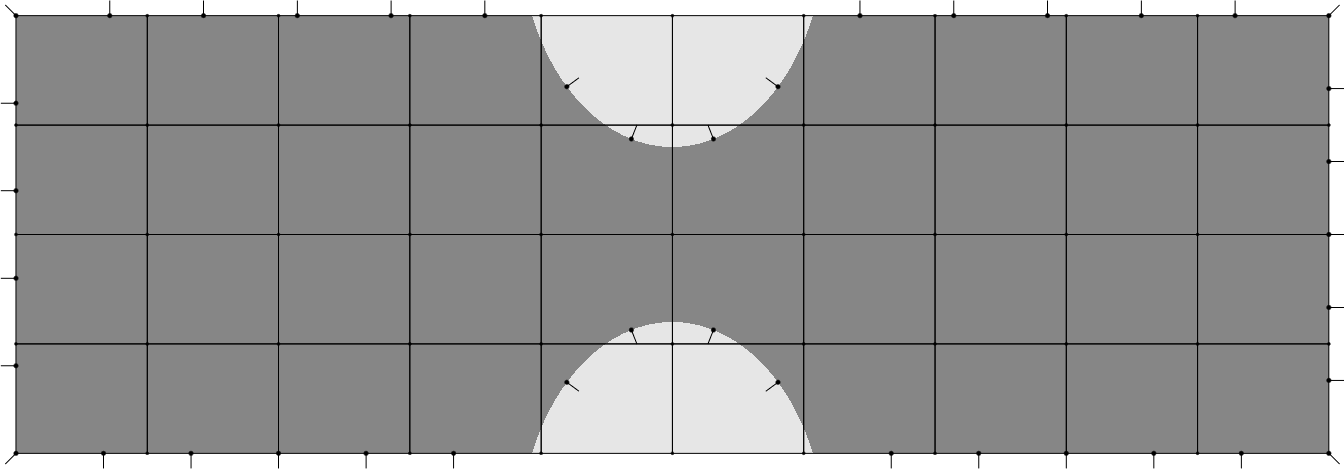
\includegraphics[width=.4\textwidth]{images/shape_opt2.png}
        \end{figure}
    \begin{itemize}
        \item Note: we can use Worst-Case Structural Analysis to
              find a loading scenario maximizing stress or deformation.
 \pause \item Say our goal is to find a visually similar object that
              is less breakage-prone (has lower combined weakness).
              \begin{itemize}
                \item Let $W(\Omega)$ be the weakness of shape $\Omega$ as measured by Worst-Case
                    Structural Analysis.
         \pause \item Assume $W$ is a differentiable function of $\Omega$ and
                    $\Omega$ can be parametrized by $p_1$...$p_k$ (e.g. CSG primitive parameters)
         \pause \item We can then compute $\frac{\partial W(\Omega)}{\partial p_i}$, the ``weakness gradient''
              \end{itemize}
         \pause \item So, if $k$ is small, something like gradient descent is reasonable
    \end{itemize}
\end{frame}

\begin{frame}{Problems: Discontinuity}
    \begin{itemize}
        \item $W$ is not a continuous function of $\Omega$; it's only piecewise continuous!
        \begin{figure}
            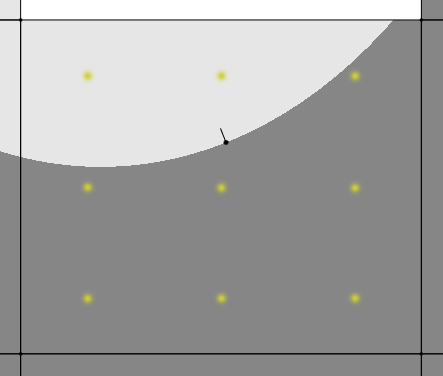
\includegraphics[width=.35\textwidth]{images/discontinuity1.png} \quad
            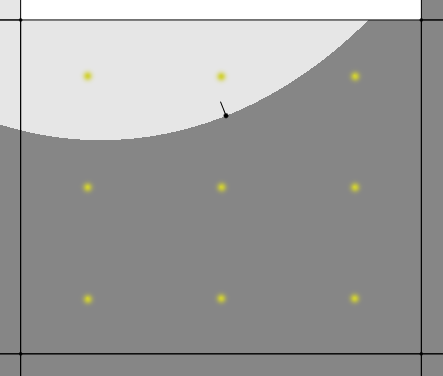
\includegraphics[width=.35\textwidth]{images/discontinuity2.png}
        \end{figure}
        (``Perceived'' geometry only changes when different quadrature points are covered)
    \end{itemize}
\end{frame}

\begin{frame}{Problems: Infinite Stress}
    \begin{itemize}
     \item Even worse, in the continuous formulation, $W$ is often infinite!
     \begin{figure}
         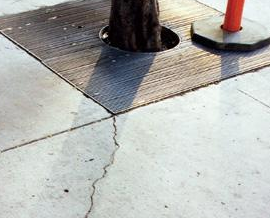
\includegraphics[height = .25\textheight]{images/re_entrant1.png} \quad
         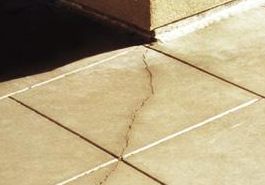
\includegraphics[height = .25\textheight]{images/re_entrant2.png}
         \caption{At a ``re-entrant'' (concave) corner, stress is infinite.}
         \source{concreteconstruction.net}
     \end{figure}
\pause \item As the grid refines around these areas, stress diverges.
\pause \item Small changes in how corners overlap the grid can vary cell stress
          averages dramatically $\Rightarrow$ amplifies discontinuity in W.
\pause \item Note: boundary-conforming (e.g. tet) meshes don't have this problem
        since the corner isn't interior.
    \end{itemize}
\end{frame}

\begin{frame}{Re-entrant Corner}
        \begin{figure}
            
\includegraphics[width=.26\textwidth]{StressRefinement/pie_90/frame_1.png} \quad
            
\includegraphics[width=.41\textwidth]{StressRefinement/pie_90/plot_1.pdf} \\
            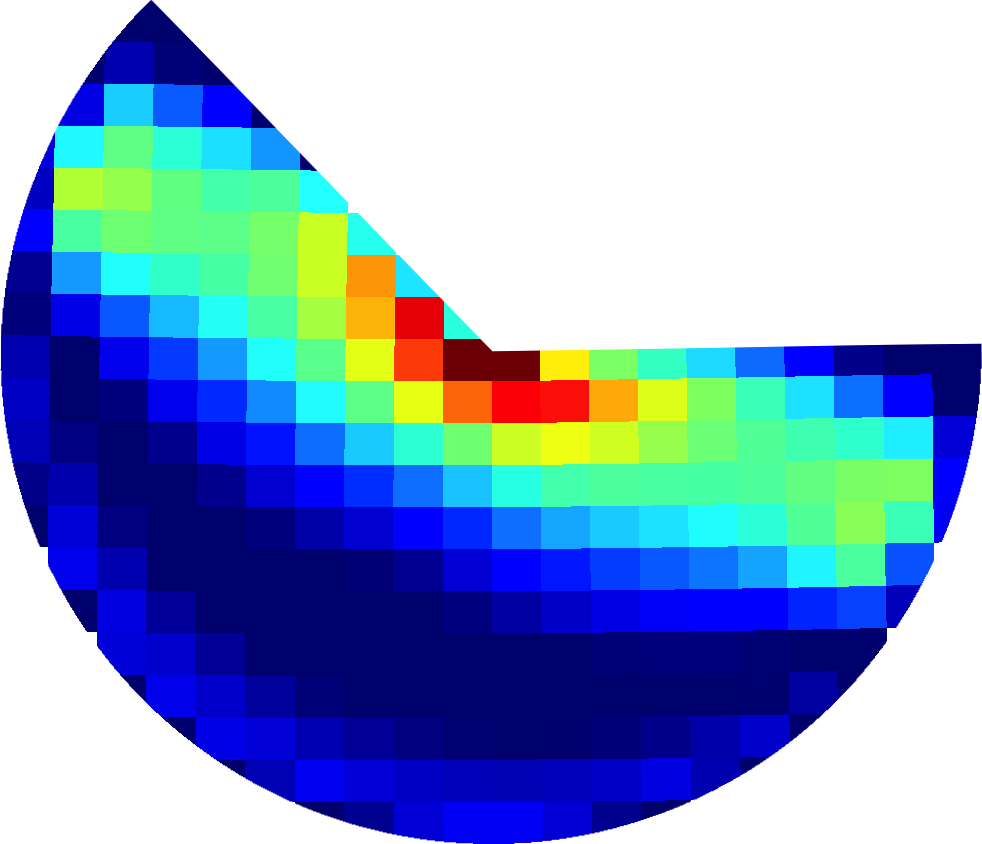
\includegraphics[width=.26\textwidth]{StressRefinement/pie_135/frame_1.png} \quad
            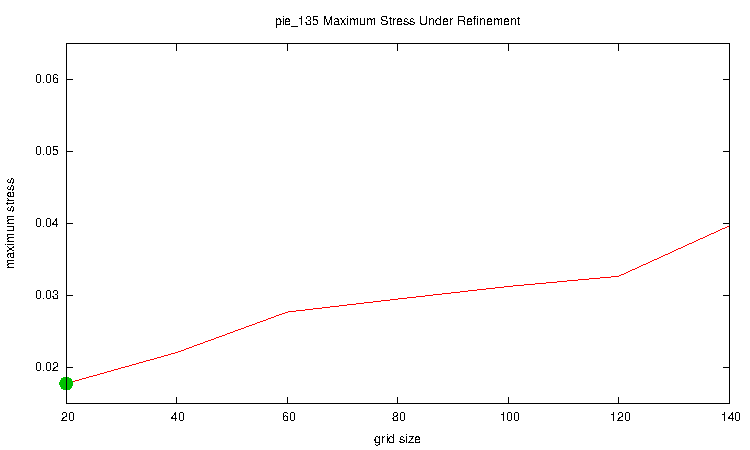
\includegraphics[width=.41\textwidth]{StressRefinement/pie_135/plot_1.pdf} \\
            \raisebox{.05\textwidth}{
\includegraphics[width=.26\textwidth]{StressRefinement/pie_180/frame_1.png}} \quad
            
\includegraphics[width=.41\textwidth]{StressRefinement/pie_180/plot_1.pdf} \\
        \end{figure}
\end{frame}

\begin{frame}{Re-entrant Corner}
        \begin{figure}
            
\includegraphics[width=.26\textwidth]{StressRefinement/pie_90/frame_2.png} \quad
            
\includegraphics[width=.41\textwidth]{StressRefinement/pie_90/plot_2.pdf} \\
            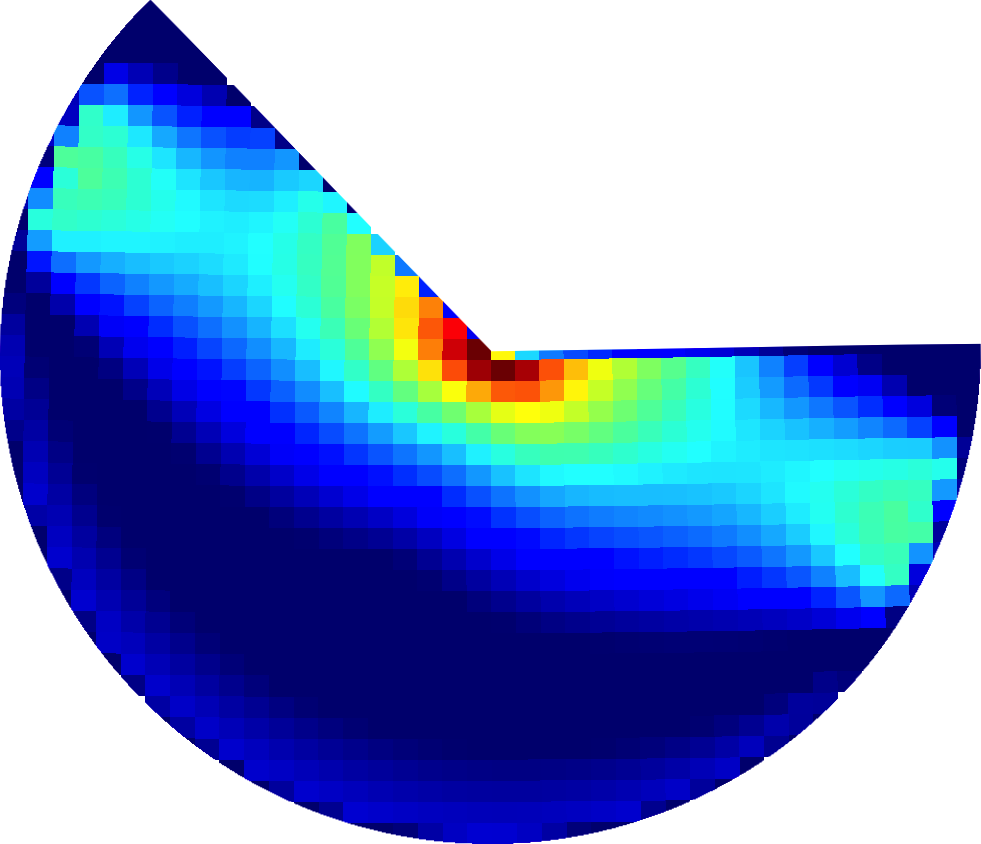
\includegraphics[width=.26\textwidth]{StressRefinement/pie_135/frame_2.png} \quad
            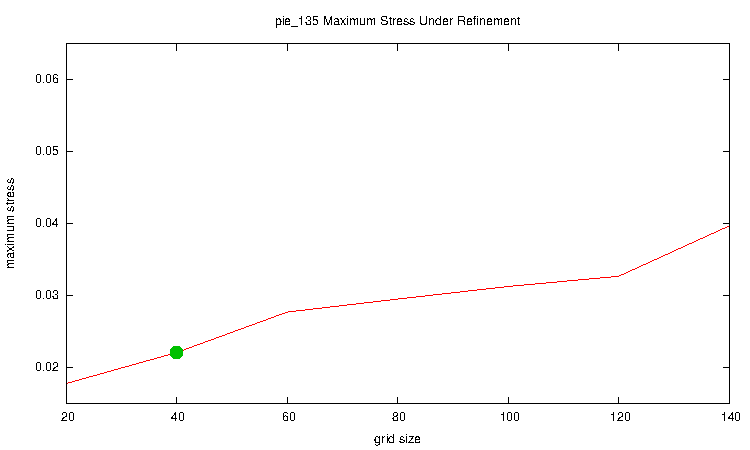
\includegraphics[width=.41\textwidth]{StressRefinement/pie_135/plot_2.pdf} \\
            \raisebox{.05\textwidth}{
\includegraphics[width=.26\textwidth]{StressRefinement/pie_180/frame_2.png}} \quad
            
\includegraphics[width=.41\textwidth]{StressRefinement/pie_180/plot_2.pdf} \\
        \end{figure}
\end{frame}

\begin{frame}{Re-entrant Corner}
        \begin{figure}
            
\includegraphics[width=.26\textwidth]{StressRefinement/pie_90/frame_3.png} \quad
            
\includegraphics[width=.41\textwidth]{StressRefinement/pie_90/plot_3.pdf} \\
            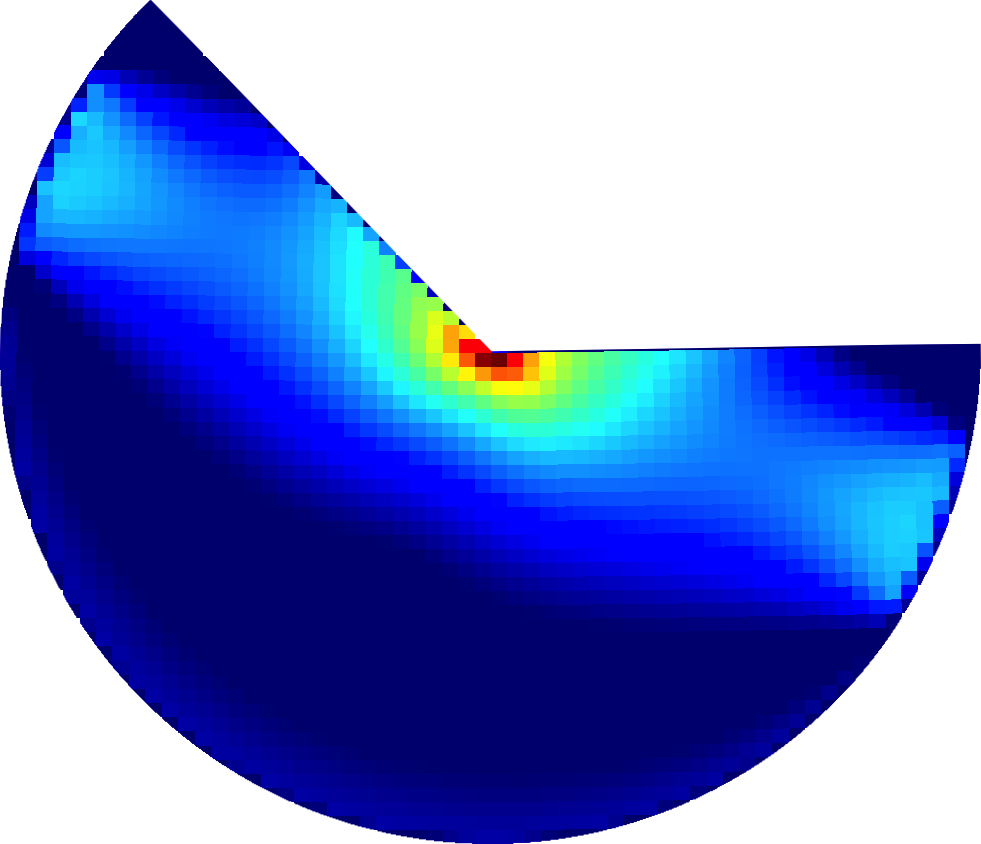
\includegraphics[width=.26\textwidth]{StressRefinement/pie_135/frame_3.png} \quad
            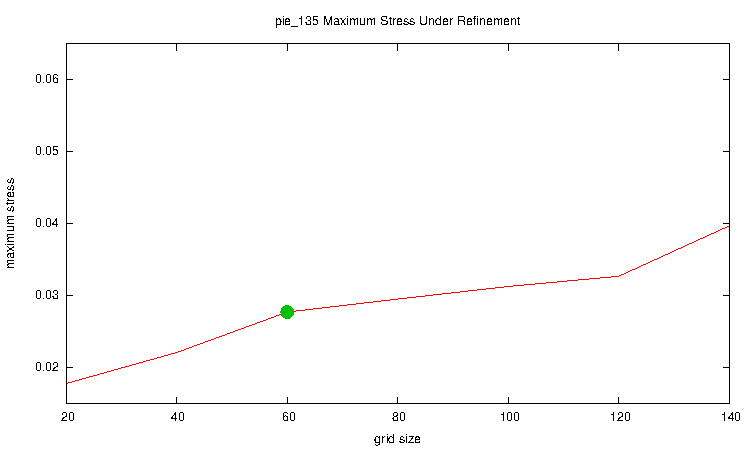
\includegraphics[width=.41\textwidth]{StressRefinement/pie_135/plot_3.pdf} \\
            \raisebox{.05\textwidth}{
\includegraphics[width=.26\textwidth]{StressRefinement/pie_180/frame_3.png}} \quad
            
\includegraphics[width=.41\textwidth]{StressRefinement/pie_180/plot_3.pdf} \\
        \end{figure}
\end{frame}

\begin{frame}{Re-entrant Corner}
        \begin{figure}
            
\includegraphics[width=.26\textwidth]{StressRefinement/pie_90/frame_4.png} \quad
            
\includegraphics[width=.41\textwidth]{StressRefinement/pie_90/plot_4.pdf} \\
            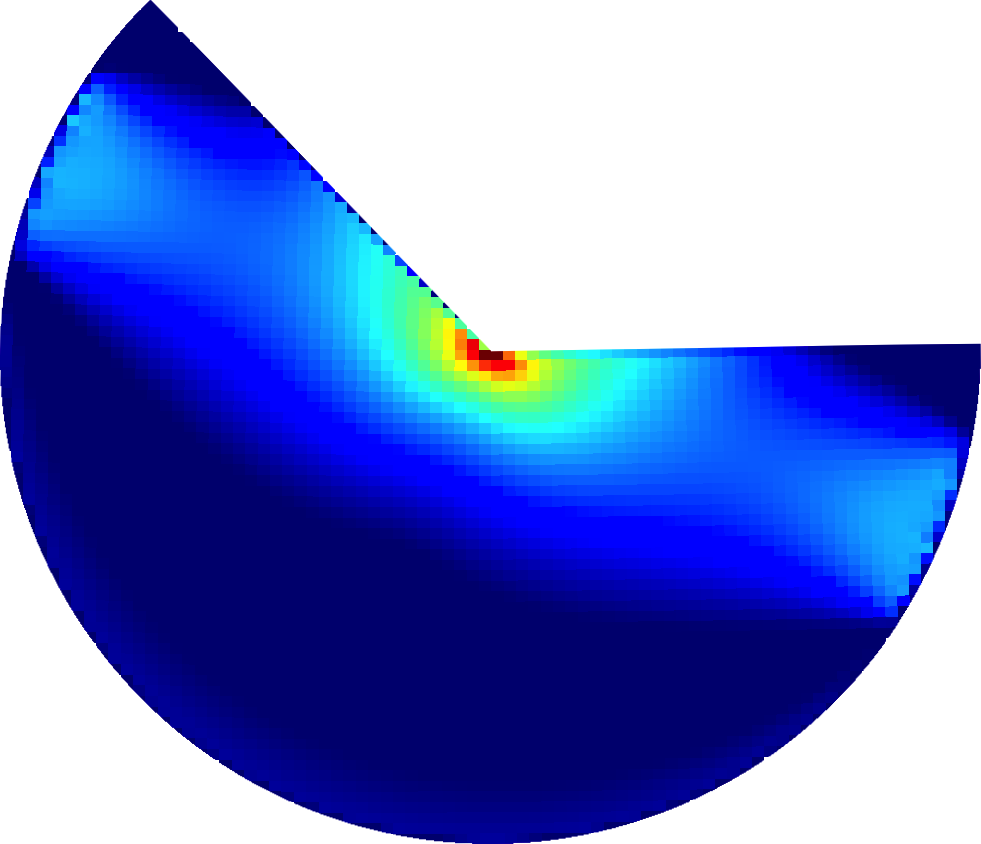
\includegraphics[width=.26\textwidth]{StressRefinement/pie_135/frame_4.png} \quad
            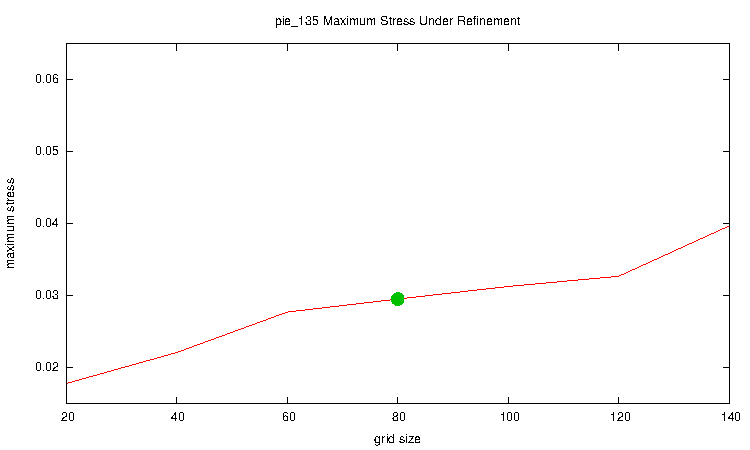
\includegraphics[width=.41\textwidth]{StressRefinement/pie_135/plot_4.pdf} \\
            \raisebox{.05\textwidth}{
\includegraphics[width=.26\textwidth]{StressRefinement/pie_180/frame_4.png}} \quad
            
\includegraphics[width=.41\textwidth]{StressRefinement/pie_180/plot_4.pdf} \\
        \end{figure}
\end{frame}

\begin{frame}{Re-entrant Corner}
        \begin{figure}
            
\includegraphics[width=.26\textwidth]{StressRefinement/pie_90/frame_5.png} \quad
            
\includegraphics[width=.41\textwidth]{StressRefinement/pie_90/plot_5.pdf} \\
            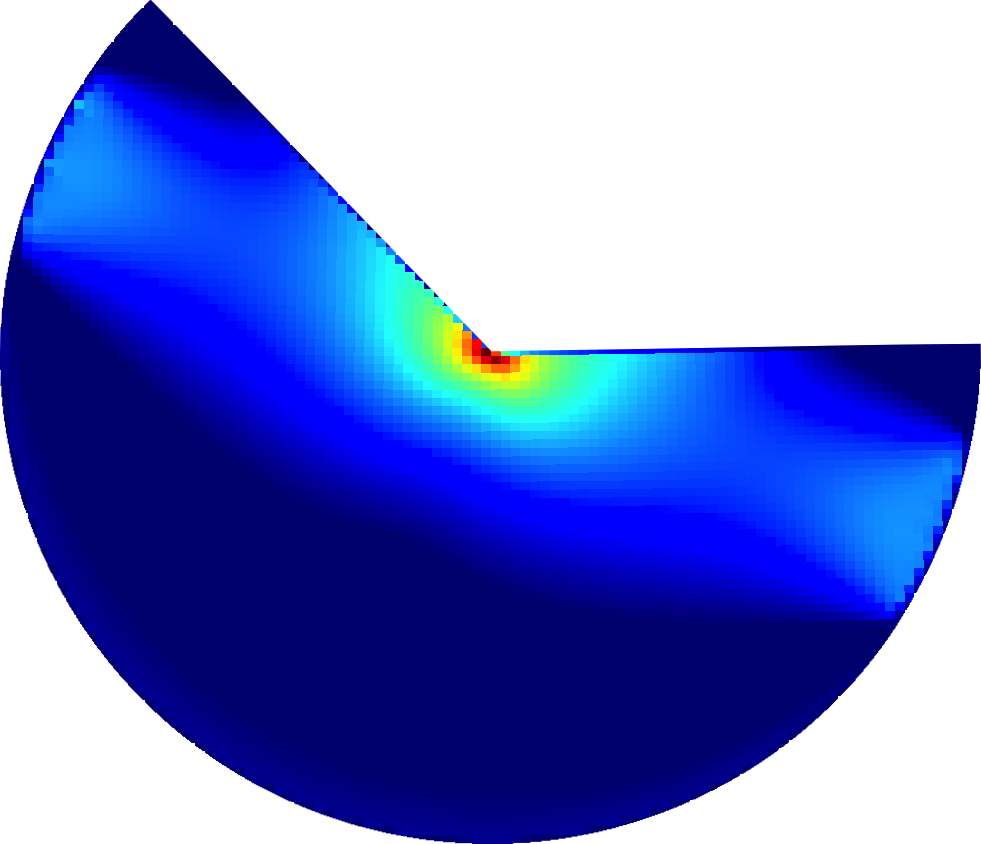
\includegraphics[width=.26\textwidth]{StressRefinement/pie_135/frame_5.png} \quad
            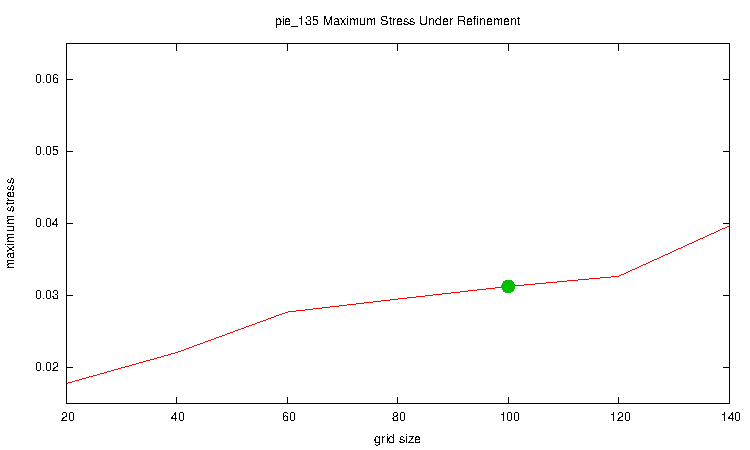
\includegraphics[width=.41\textwidth]{StressRefinement/pie_135/plot_5.pdf} \\
            \raisebox{.05\textwidth}{
\includegraphics[width=.26\textwidth]{StressRefinement/pie_180/frame_5.png}} \quad
            
\includegraphics[width=.41\textwidth]{StressRefinement/pie_180/plot_5.pdf} \\
        \end{figure}
\end{frame}

\begin{frame}{Re-entrant Corner}
        \begin{figure}
            
\includegraphics[width=.26\textwidth]{StressRefinement/pie_90/frame_6.png} \quad
            
\includegraphics[width=.41\textwidth]{StressRefinement/pie_90/plot_6.pdf} \\
            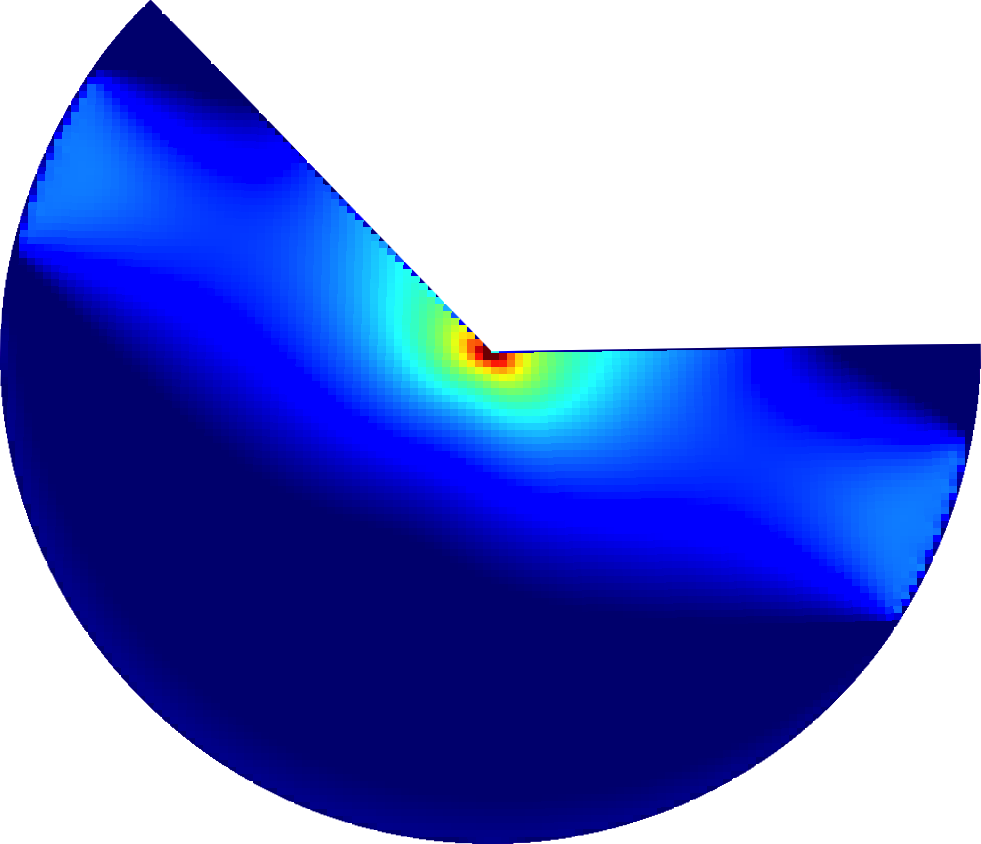
\includegraphics[width=.26\textwidth]{StressRefinement/pie_135/frame_6.png} \quad
            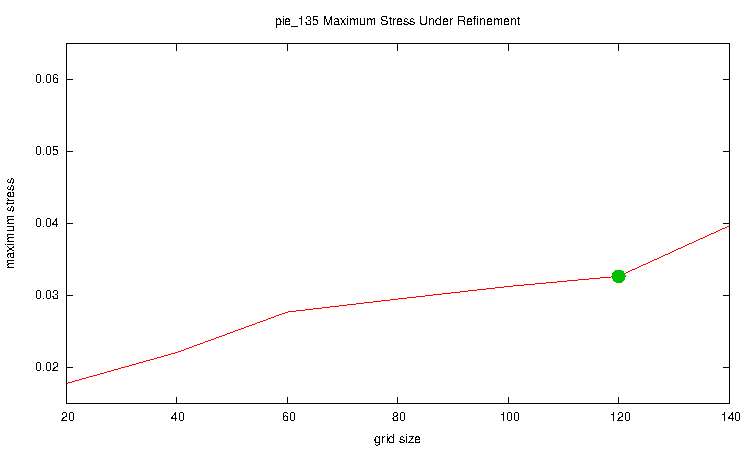
\includegraphics[width=.41\textwidth]{StressRefinement/pie_135/plot_6.pdf} \\
            \raisebox{.05\textwidth}{
\includegraphics[width=.26\textwidth]{StressRefinement/pie_180/frame_6.png}} \quad
            
\includegraphics[width=.41\textwidth]{StressRefinement/pie_180/plot_6.pdf} \\
        \end{figure}
\end{frame}

\begin{frame}{Re-entrant Corner}
        \begin{figure}
            
\includegraphics[width=.26\textwidth]{StressRefinement/pie_90/frame_7.png} \quad
            
\includegraphics[width=.41\textwidth]{StressRefinement/pie_90/plot_7.pdf} \\
            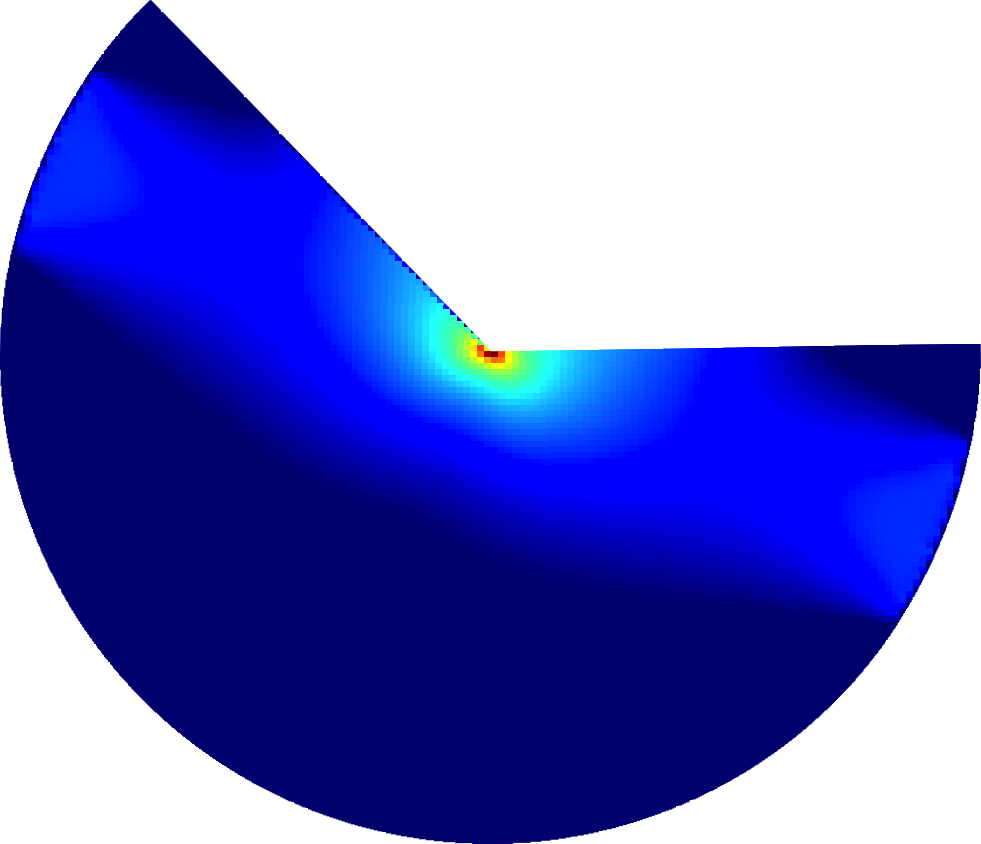
\includegraphics[width=.26\textwidth]{StressRefinement/pie_135/frame_7.png} \quad
            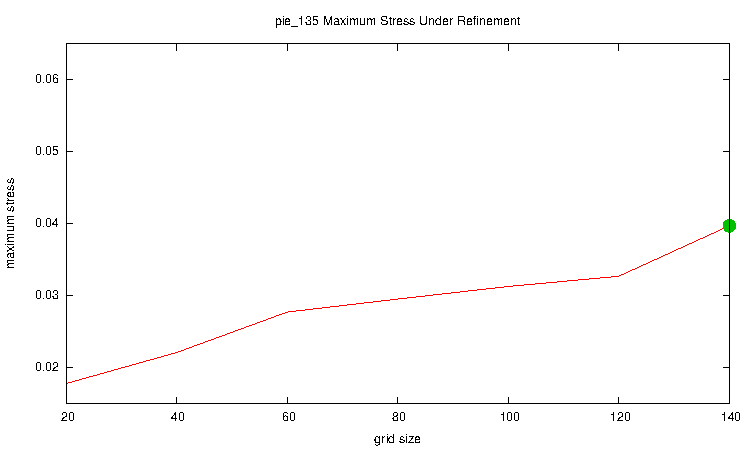
\includegraphics[width=.41\textwidth]{StressRefinement/pie_135/plot_7.pdf} \\
            \raisebox{.05\textwidth}{
\includegraphics[width=.26\textwidth]{StressRefinement/pie_180/frame_7.png}} \quad
            
\includegraphics[width=.41\textwidth]{StressRefinement/pie_180/plot_7.pdf} \\
        \end{figure}
\end{frame}

\begin{frame}{Avoiding These Problems}
    \begin{itemize}
        \item Avoid diverging stress by computing average stress over a fixed
              region instead of per-element stress (should converge under
              refinement).
      \pause \item
          Use a signed distance function to blur the object (replace
          discontinuous $I_\Omega$ with smooth function).
          \begin{itemize}
              \item Demo
            \pause \item Now, $W$ will be a continuous function of $p_i$
            \pause \item $W$ should be differentiable if a differentiable
                approximation to the signed distance function is used
                (R-functions)
          \end{itemize}
    \end{itemize}
\end{frame}

\end{document}
